
\section{Implementation}
\label{sec:implementation}

In this section, we details our implementation on Arduino \cite{Arduino} platform. The whole system is comprised of a glass module, numbers of clients, and a gateway. We will start by the clients, for which we only implement the simpliest functionalities. We push the burden of coordination to the glass.

\subsection{Clients}
The clients are comprised of a main Arduino board, an IR receiver, an XBee radio, and various actuators. In our current system, we have a relay which can control the AC power plug, and we have a USB connected computer to control video playing. 

The main function of client is to respond IR signal, and communicate with glass to receive corresponding commands. When there is no glass initiating connection, the client simply lives in {\it IDLE} mode; while when they receive IR signal, indicating the user is expressing interest in interacting with it, the client responds with an XBee acknowledgement and goes into {\it PENDING} state. In this case, since the client doesn't know how many other clients have also responded to the glass, it will wait until a connection signal. If there are multiple clients waiting to be verified, the glass will coordinate all of them by sending the right verifying message. The active client that is being verified will blink faster, as visual feedback to users. When it receives the connection message, it goes to {\it CONNECTED} state and is ready to take commands. To summarize the behavior, we have a state machine in Fig.\,\ref{fig:clientFSM} for illustration. 

\begin{figure}
  \centering
  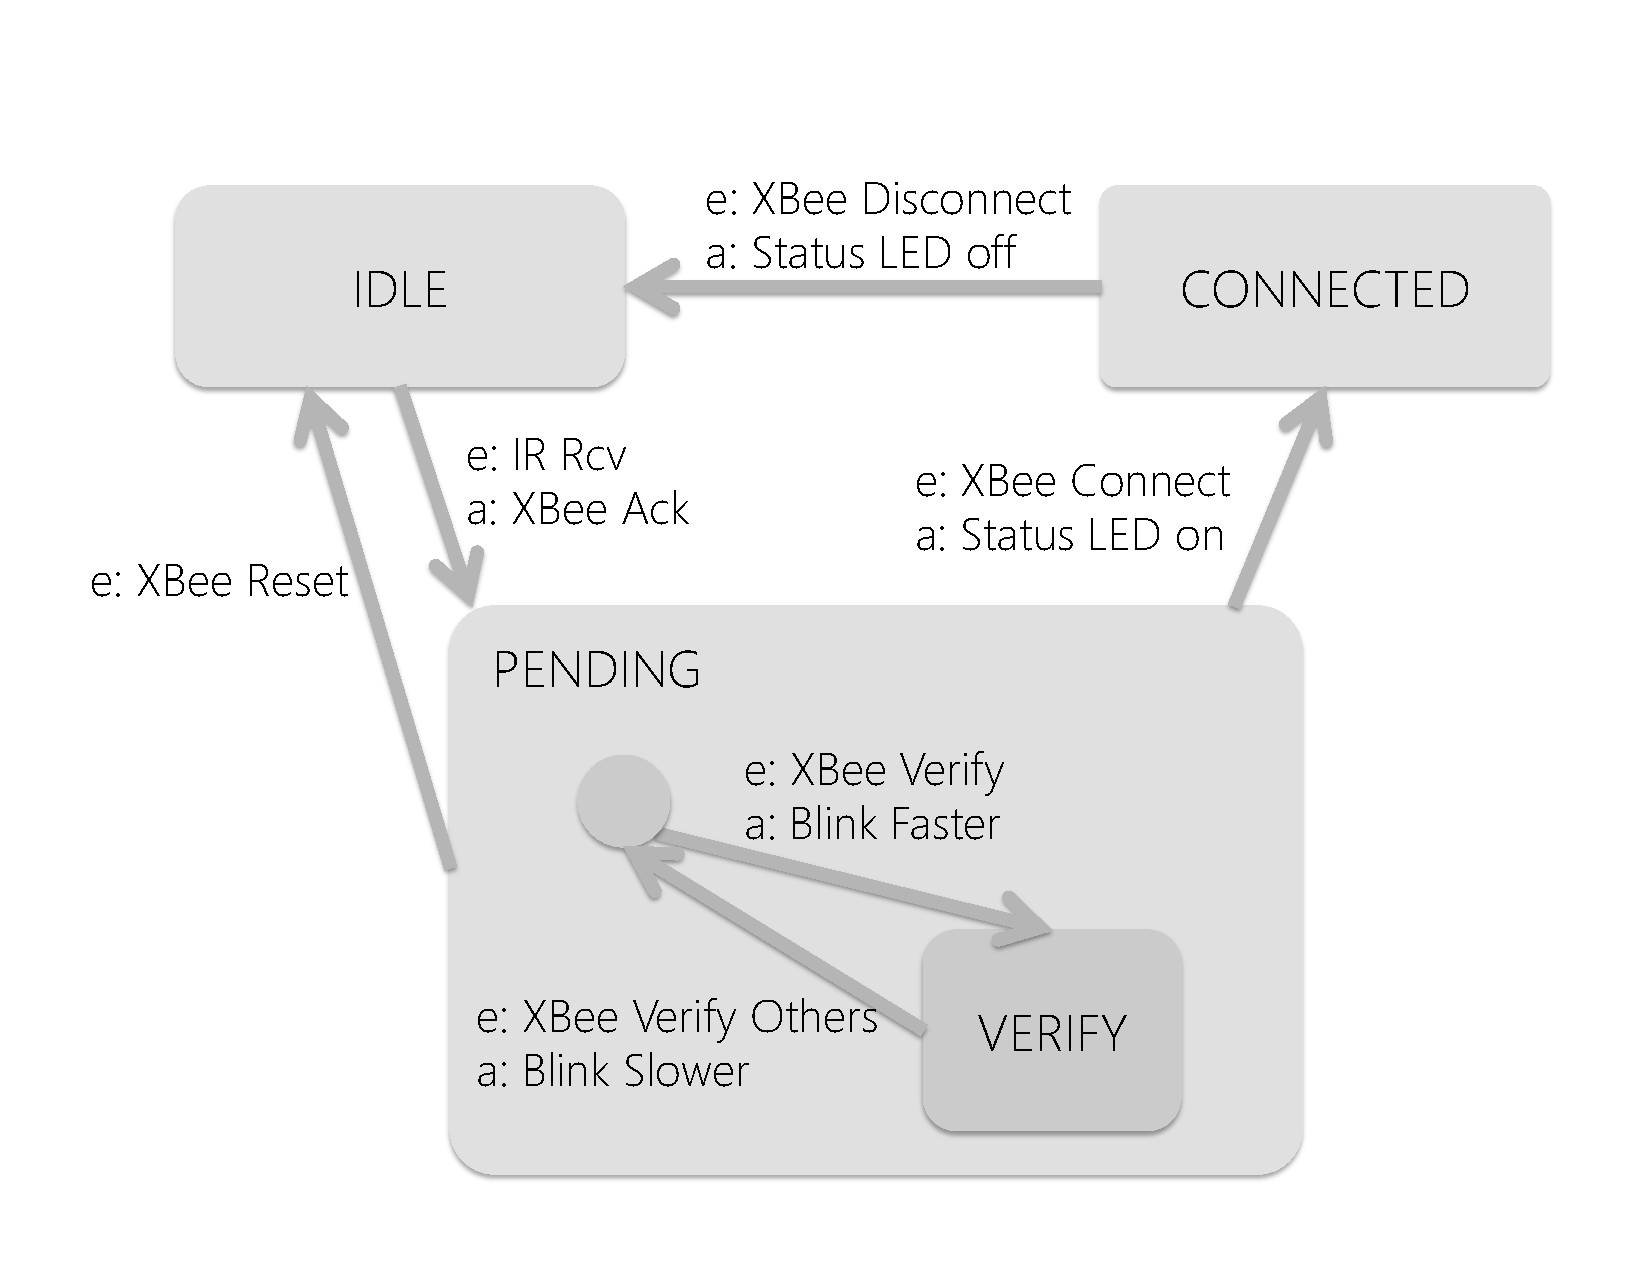
\includegraphics[width=\linewidth]{../figs/clientFSM.pdf}
  \caption{FSM model for client}
  \label{fig:clientFSM}
\end{figure}

Within {\it CONNECTED} state, the clients' behaviors are different from each other according to the device it is connected to. In our prototype, we have two different types of devices. The first is a relay, which can then control the whole AC power supply. To control the relay, we only need to set a digital pin to {\it LOW} or {\it HIGH}, and each action is encoded in the command set from the glass. The second is a computer that is used to play video. And the direct interaction includes adjusting the volume and pause/play. These commands are sent to the computer through USB serial data.

\subsection{Glass}
\label{sec:glass}

The Glass is complicated in two folds. First, we move the complexity of coordinating all clients to the Glass. Second, we have to handle user gesture on Glass. 

% add graphs and FSM for Glass

\subsection{Gateway}
\label{sec:gateway}

The gateway provides access to the personal area network for computers, and presumably this can be further open to the Internet. Since there have already been many products \cite{NinjaBlocks, Lockitron} that essentially function in this way, we do not spend much time on this aspect in our project. 



%%% Local Variables: 
%%% mode: latex
%%% TeX-master: "main"
%%% End: 
